% Options for packages loaded elsewhere
\PassOptionsToPackage{unicode}{hyperref}
\PassOptionsToPackage{hyphens}{url}
%
\documentclass[
  man]{apa6}
\usepackage{amsmath,amssymb}
\usepackage{lmodern}
\usepackage{iftex}
\ifPDFTeX
  \usepackage[T1]{fontenc}
  \usepackage[utf8]{inputenc}
  \usepackage{textcomp} % provide euro and other symbols
\else % if luatex or xetex
  \usepackage{unicode-math}
  \defaultfontfeatures{Scale=MatchLowercase}
  \defaultfontfeatures[\rmfamily]{Ligatures=TeX,Scale=1}
\fi
% Use upquote if available, for straight quotes in verbatim environments
\IfFileExists{upquote.sty}{\usepackage{upquote}}{}
\IfFileExists{microtype.sty}{% use microtype if available
  \usepackage[]{microtype}
  \UseMicrotypeSet[protrusion]{basicmath} % disable protrusion for tt fonts
}{}
\makeatletter
\@ifundefined{KOMAClassName}{% if non-KOMA class
  \IfFileExists{parskip.sty}{%
    \usepackage{parskip}
  }{% else
    \setlength{\parindent}{0pt}
    \setlength{\parskip}{6pt plus 2pt minus 1pt}}
}{% if KOMA class
  \KOMAoptions{parskip=half}}
\makeatother
\usepackage{xcolor}
\usepackage{graphicx}
\makeatletter
\def\maxwidth{\ifdim\Gin@nat@width>\linewidth\linewidth\else\Gin@nat@width\fi}
\def\maxheight{\ifdim\Gin@nat@height>\textheight\textheight\else\Gin@nat@height\fi}
\makeatother
% Scale images if necessary, so that they will not overflow the page
% margins by default, and it is still possible to overwrite the defaults
% using explicit options in \includegraphics[width, height, ...]{}
\setkeys{Gin}{width=\maxwidth,height=\maxheight,keepaspectratio}
% Set default figure placement to htbp
\makeatletter
\def\fps@figure{htbp}
\makeatother
\setlength{\emergencystretch}{3em} % prevent overfull lines
\providecommand{\tightlist}{%
  \setlength{\itemsep}{0pt}\setlength{\parskip}{0pt}}
\setcounter{secnumdepth}{-\maxdimen} % remove section numbering
% Make \paragraph and \subparagraph free-standing
\ifx\paragraph\undefined\else
  \let\oldparagraph\paragraph
  \renewcommand{\paragraph}[1]{\oldparagraph{#1}\mbox{}}
\fi
\ifx\subparagraph\undefined\else
  \let\oldsubparagraph\subparagraph
  \renewcommand{\subparagraph}[1]{\oldsubparagraph{#1}\mbox{}}
\fi
\newlength{\cslhangindent}
\setlength{\cslhangindent}{1.5em}
\newlength{\csllabelwidth}
\setlength{\csllabelwidth}{3em}
\newlength{\cslentryspacingunit} % times entry-spacing
\setlength{\cslentryspacingunit}{\parskip}
\newenvironment{CSLReferences}[2] % #1 hanging-ident, #2 entry spacing
 {% don't indent paragraphs
  \setlength{\parindent}{0pt}
  % turn on hanging indent if param 1 is 1
  \ifodd #1
  \let\oldpar\par
  \def\par{\hangindent=\cslhangindent\oldpar}
  \fi
  % set entry spacing
  \setlength{\parskip}{#2\cslentryspacingunit}
 }%
 {}
\usepackage{calc}
\newcommand{\CSLBlock}[1]{#1\hfill\break}
\newcommand{\CSLLeftMargin}[1]{\parbox[t]{\csllabelwidth}{#1}}
\newcommand{\CSLRightInline}[1]{\parbox[t]{\linewidth - \csllabelwidth}{#1}\break}
\newcommand{\CSLIndent}[1]{\hspace{\cslhangindent}#1}
\ifLuaTeX
\usepackage[bidi=basic]{babel}
\else
\usepackage[bidi=default]{babel}
\fi
\babelprovide[main,import]{english}
% get rid of language-specific shorthands (see #6817):
\let\LanguageShortHands\languageshorthands
\def\languageshorthands#1{}
% Manuscript styling
\usepackage{upgreek}
\captionsetup{font=singlespacing,justification=justified}

% Table formatting
\usepackage{longtable}
\usepackage{lscape}
% \usepackage[counterclockwise]{rotating}   % Landscape page setup for large tables
\usepackage{multirow}		% Table styling
\usepackage{tabularx}		% Control Column width
\usepackage[flushleft]{threeparttable}	% Allows for three part tables with a specified notes section
\usepackage{threeparttablex}            % Lets threeparttable work with longtable

% Create new environments so endfloat can handle them
% \newenvironment{ltable}
%   {\begin{landscape}\centering\begin{threeparttable}}
%   {\end{threeparttable}\end{landscape}}
\newenvironment{lltable}{\begin{landscape}\centering\begin{ThreePartTable}}{\end{ThreePartTable}\end{landscape}}

% Enables adjusting longtable caption width to table width
% Solution found at http://golatex.de/longtable-mit-caption-so-breit-wie-die-tabelle-t15767.html
\makeatletter
\newcommand\LastLTentrywidth{1em}
\newlength\longtablewidth
\setlength{\longtablewidth}{1in}
\newcommand{\getlongtablewidth}{\begingroup \ifcsname LT@\roman{LT@tables}\endcsname \global\longtablewidth=0pt \renewcommand{\LT@entry}[2]{\global\advance\longtablewidth by ##2\relax\gdef\LastLTentrywidth{##2}}\@nameuse{LT@\roman{LT@tables}} \fi \endgroup}

% \setlength{\parindent}{0.5in}
% \setlength{\parskip}{0pt plus 0pt minus 0pt}

% Overwrite redefinition of paragraph and subparagraph by the default LaTeX template
% See https://github.com/crsh/papaja/issues/292
\makeatletter
\renewcommand{\paragraph}{\@startsection{paragraph}{4}{\parindent}%
  {0\baselineskip \@plus 0.2ex \@minus 0.2ex}%
  {-1em}%
  {\normalfont\normalsize\bfseries\itshape\typesectitle}}

\renewcommand{\subparagraph}[1]{\@startsection{subparagraph}{5}{1em}%
  {0\baselineskip \@plus 0.2ex \@minus 0.2ex}%
  {-\z@\relax}%
  {\normalfont\normalsize\itshape\hspace{\parindent}{#1}\textit{\addperi}}{\relax}}
\makeatother

% \usepackage{etoolbox}
\makeatletter
\patchcmd{\HyOrg@maketitle}
  {\section{\normalfont\normalsize\abstractname}}
  {\section*{\normalfont\normalsize\abstractname}}
  {}{\typeout{Failed to patch abstract.}}
\patchcmd{\HyOrg@maketitle}
  {\section{\protect\normalfont{\@title}}}
  {\section*{\protect\normalfont{\@title}}}
  {}{\typeout{Failed to patch title.}}
\makeatother

\usepackage{xpatch}
\makeatletter
\xapptocmd\appendix
  {\xapptocmd\section
    {\addcontentsline{toc}{section}{\appendixname\ifoneappendix\else~\theappendix\fi\\: #1}}
    {}{\InnerPatchFailed}%
  }
{}{\PatchFailed}
\keywords{keywords\newline\indent Word count: X}
\DeclareDelayedFloatFlavor{ThreePartTable}{table}
\DeclareDelayedFloatFlavor{lltable}{table}
\DeclareDelayedFloatFlavor*{longtable}{table}
\makeatletter
\renewcommand{\efloat@iwrite}[1]{\immediate\expandafter\protected@write\csname efloat@post#1\endcsname{}}
\makeatother
\usepackage{csquotes}
\ifLuaTeX
  \usepackage{selnolig}  % disable illegal ligatures
\fi
\IfFileExists{bookmark.sty}{\usepackage{bookmark}}{\usepackage{hyperref}}
\IfFileExists{xurl.sty}{\usepackage{xurl}}{} % add URL line breaks if available
\urlstyle{same} % disable monospaced font for URLs
\hypersetup{
  pdftitle={Are bond price predictible?},
  pdfauthor={Saurav Mawandia1 \& Sougandh Kohli1},
  pdflang={en-EN},
  pdfkeywords={keywords},
  hidelinks,
  pdfcreator={LaTeX via pandoc}}

\title{Are bond price predictible?}
\author{Saurav Mawandia\textsuperscript{1} \& Sougandh Kohli\textsuperscript{1}}
\date{}


\shorttitle{Predicting bond price using Deep Learning}

\authornote{

The authors made the following contributions. Saurav Mawandia: Conceptualization, Writing - Original Draft Preparation, Writing - Review \& Editing; Sougandh Kohli: Conceptualization, Writing - Original Draft Preparation, Writing - Review \& Editing.

Correspondence concerning this article should be addressed to Saurav Mawandia, 326 Market St, Harrisburg, PA 17101. E-mail: \href{mailto:smawandia@my.harrisburgu.edu}{\nolinkurl{smawandia@my.harrisburgu.edu}}

}

\affiliation{\vspace{0.5cm}\textsuperscript{1} Harrisburg University of Science and Technology}

\abstract{%
The capital market plays a crucial role in the development of a country. The overall size of the global bond market as of 2021 is over 128.3tn. In contrast, the overall size of the equities market is 44 trillion as of 2022. However, the bond market is not much transparent compared to stock, and only a few firms try to predict the price of bonds. Different brokers can give different prices for the same bond, making it challenging for anyone to predict the bond's price based on these data. A bond is usually based on the last traded price and indicative bids and asks.
Moreover, predicting the price of a bond thus becomes challenging. That is why it is essential to understand the overall market for bonds and consider the prices. For humans, it is tough to keep an eye on the fixed income market and make a decision. That is where Artificial Intelligent systems help us. Machine learning algorithms use the data and find hidden patterns to predict the correct price of a given bond. Given the data related to the fixed income market, news related to the market, and so on, we train an AI algorithm to predict the price of the given bond. It considers the details like rating, last traded price, type, and news around the bond to predict the right price for a trader to trade.
}



\begin{document}
\maketitle

\hypertarget{introduction}{%
\section{Introduction}\label{introduction}}

A bond valuation uses a yield to maturity or a zero yield curve using a few points on the par bond or Nelson Siegel parameters. The bond is valued using the settlement date and maturity date using an algorithm that can calculate the time to maturity and each coupon date. Maturity can be in years; if unavailable, a zero maturity date is used. This mode is particularly convenient for price par bonds or price other bonds on issue dates or coupon dates. Using this mode between coupon dates is difficult as the user has to compute the day count and year fraction and provide the maturity as, say, 5.3 years. Traditionally bond price was calculated using YTM(Yield to maturity) or zero yield curve. However, this approach does not predict an accurate price of a bond because it does not consider other parameters such as inflation. We have used the LSTM model to predict trade price based on the last trade price, which can be improved further to consider external factors such as inflation.
Long short-term memory (LSTM) is an artificial neural network in artificial intelligence. Unlike standard feedforward neural networks, LSTM has feedback connections. Such a recurrent neural network (RNN) can process not only single data points but also entire data sequences and is also suitable for analyzing time series data.

\hypertarget{background}{%
\section{Background}\label{background}}

As far as price transparency is concerned, there has historically been a huge gap between the amount of reference information available to those trading equities versus those trading corporate bonds. Stock exchanges report trades, bids and offers at all times. Free access is available online with a 15 minute delay while traders who demand more information can pay for ultra efficient real time data and information about size of current bids and offers. By contrast, bond trades are required to be reported within 15 minutes and only those who pay for the TRACE feed can access this information. No quotes are publicly available and the best way to get a quote is to solicit multiple brokers and wait for a reply. Alternatively there are data companies that provide end of day prices, published after the market has closed and with no guarantee that the specific information sought will be included. Accurate bond pricing is also hindered by lack of liquidity. Only a fraction of TRACE eligible bonds trade on a given day, so the most recent trade price is often multiple days old. Pricing bonds based on other more liquid bonds that have similar features is common, but again limited by the presence of such bonds.

\par

Thus, in the context of bond price predictions, machine learning should be fast and accurate. They have evaluated the performance of various supervised learning algorithms for regression followed by ensemble methods, with feature and model selection considerations being treated in detail(Ganguli and Dunnmon (2017)). (Götze, Gürtler, and Witowski (2020)) compares the forecasting performance of linear regression models and enhanced machine learning methods in the catastrophe (CAT) bonds market using linear regression with variable selection, penalization methods, random forests, and neural networks to forecast CAT bond premia. Random forests exhibit the highest forecasting performance among the considered models, followed by linear regression models and neural networks.

\par

Benchmark Solutions is the first provider of realtime corporate bond prices. Every 10 seconds they provide accurate prices that incorporate interest rate data, trades or quotes of the bond in question, trades or quotes of other bonds or CDS of the issuer of the bond in question as well as other input sources. Pricing bonds accurately requires an exacting knowledge of payment schedules, trading calenders and reference data for each bond. This, as well as synthesizing all of the bonds and CDS quotes and trades of a given issuer into implied hazard and funding curves, is something that they feel is beyond the scope of this challenge. (Golbayani, Florescu, and Chatterjee (2020)) Rather, they provide you with a reference price which is an intermediate result of our calculations and is labeled `curve\_based\_price' in the dataset. Thus the competition focuses on trading dynamics and microstructure of individual bonds, rather than all bonds from a given issuer. (Ganguli and Dunnmon (2017)) proposes a novel hybrid time-series aided machine learning method that could be applied to such datasets in future work.

\par

Benchmark solutions are the first provider of real-time corporate bond prices discussed in (Bacas (2018)). Every 10 seconds, they provide accurate prices that incorporate interest rate data, trades or quotes of the bond in question, trades or quotes of other bonds or CDS of the issuer of the bond in question, and other input sources. Pricing bonds accurately requires exacting knowledge of payment schedules, trading calendars, and reference data for each bond. This, as well as synthesizing all of the bonds and CDS quotes and trades of a given issuer into the implied hazard and funding curves, is something that we feel is beyond the scope of this challenge. Rather, we provide you with a reference price which is an intermediate result of our calculations and is labeled `curve\_based\_price' in the dataset. Thus the competition focuses on trading dynamics and microstructure of individual bonds rather than all bonds from a given issuer.

\hypertarget{methods}{%
\section{Methods}\label{methods}}

This research paper's methodology focuses on quantitative aspects of bond price prediction. These variables are not the extent of dependency but have provided a credible amount of accuracy in the past to other researchers. Simple linear regression and Long Short Term model (LSTM) are used to estimate the prices using the significantly important variables. LSTM proved to be more effective for sequential data.

\hypertarget{data}{%
\subsection{Data}\label{data}}

The dataset is downloaded from Kaggle. US corporate bond trade data is provided. Each row includes trade details, some basic information about the traded bond, and information about the previous ten trades. The data is discussed below. There are 3736 unique bonds present in the data. While we can use this as one Id in the real world, there is no bond\_id in the test.csv file, so we can either prepare data using it or drop it. But, dropping bond\_id is losing meaningful info, so we will create one function we can use for each bond Id to construct time-series data for it, and then we will train some models on it.
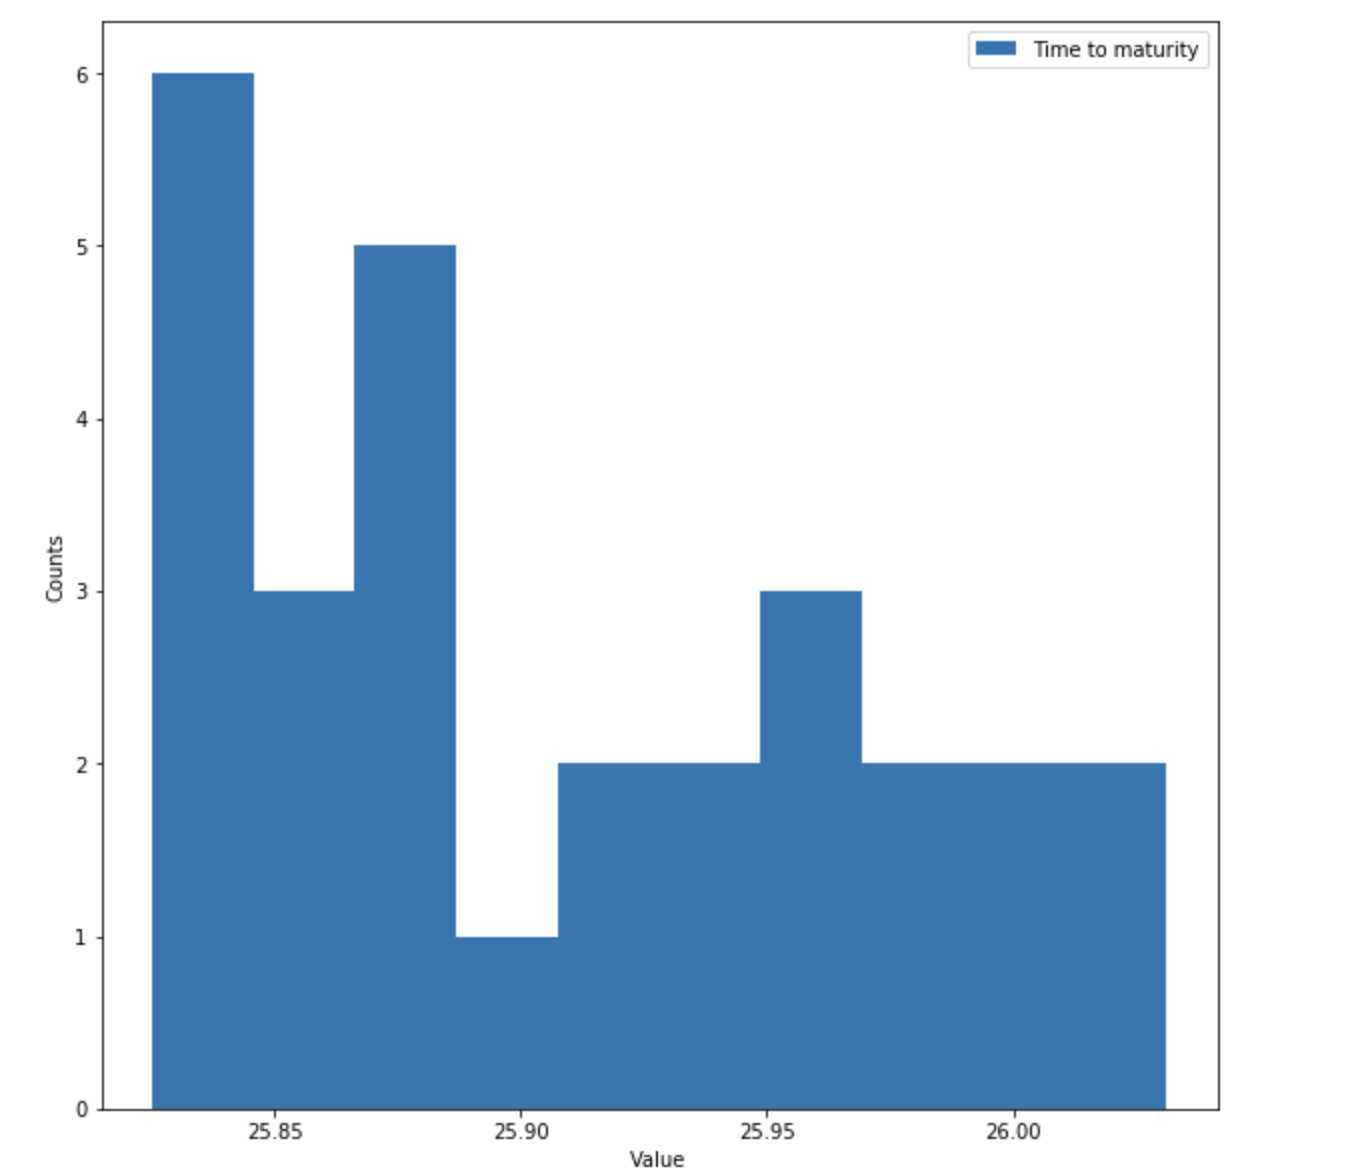
\includegraphics{timeTomaturity.png}
The above plot shows how the maturity time is distributed for a given bond. Sometimes it is helpful to decide which type of bonds have a high maturity time and which have less; The bond price can change a lot based on that.

\begin{itemize}
\tightlist
\item
  id: The row id. bond\_id: The unique id of a bond to aid in time series reconstruction. (This column is only present in the train data). 3736 unique bond ids, varying from 12,129 data points to 1 per id.
\item
  trade\_price: The price at which the trade occurred. (This is the column to predict in the test data). Mean: 103.44, Median: 102.33, STD: 9.82.
\item
  weight: The weight of the row for evaluation purposes. This is calculated as the square root of the time since the last trade and then scaled so the mean is 1.
\item
  current\_coupon: The coupon of the bond at the time of the trade.
\item
  time\_to\_maturity: The number of years until the bond matures at the time of the trade.
\item
  curve\_based\_price: A fair price estimate based on implied hazard and funding curves of the issuer of the bond.
\item
  reporting\_delay: The number of seconds after the trade occurred that it was reported.
\item
  trade\_size: The notional amount of the trade.
\end{itemize}

\hypertarget{procedure}{%
\subsection{Procedure}\label{procedure}}

We can not use the id column at all. So we drop it first. Then we create one function to take our data frame and construct time series data from it. It means that the next trade price will be the output for the current trade. This way, we provide the existing data to predict the next trade price. We have more than 3000 unique bonds. So for all of those bonds, we have to construct the time series data. So, we group by object and then apply our function to create the time-series data. Then we combine all the data into one data frame for further usage. The above data frame has our last column as output. We do not need the bond\_id column as it has no valuable information for us. Also, this column is not present in the test.csv file for the competition. So, we try to look closely at the competition data. Then, we scale the data from 0 to 1. This way, our model can fit the data best as normalized. Finally, it is time to split the data into train and test data. We will use 90\% of the data to train the model and the rest 10\% for testing our model. We will use the LSTM model to reshape our data as per the required shape of the LSTM.

\par

Now we build our model. We are using the Keras library, which is running on top of TensorFlow. We create a simple LSTM model with one LSTM and one Dense layer for output. In the output layer, we use linear activation as our final output is price, which is float. Now, it is time to train the model. Now, as our model is trained, let's test it. We make predictions on the test data and then check out the root mean square error of the predictions. In doing so, we also need to convert the normalized data into raw data. We can do this by using MinMaxScaler inverse\_transform function. The above-predicted prices are close to the accurate prices. Of course, there can be chances of data leakage or some other issue like the overfitting of the model. But, it shows us the LSTM network's potential to predict the bond trade price given the historical data.

\hypertarget{data-analysis}{%
\subsection{Data analysis}\label{data-analysis}}

After seeing the results of (Ganguli and Dunnmon (2017)) we decided to assert most of our efforts into developing RNN-LSTM or Long Short-Term Memory Neural Network. LSTMs are great for working with time series data as their weights are longer depending on time series lag. However, this can substantially slow down the processing speed by having to save these specific weights, which was the case with this model. It took well over 5 hours to reach convergence.

\hypertarget{results}{%
\section{Results}\label{results}}

An essential aspect of these results is the consideration of speed AND accuracy. Benchmark Solutions wanted actionable information which could be fast and effective. LSTM NN which came close to the first NN in accuracy but took substantially longer to run, reaching convergence at just over 100 epochs taking 5 hours and 22 minutes. The result below shows us that our predicted price was very close to the real trade price.

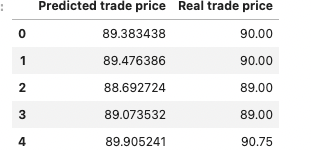
\includegraphics{result.png}

\hypertarget{discussion-future-work}{%
\section{Discussion/ Future work}\label{discussion-future-work}}

In the testing process, we were limited by computing processing capability. First, we started using data bricks, which was also very slow. Next, we ran on both GPU and CPU, which improved our testing times but was still a substantial barrier to adjusting our tests. Further, improved computational power would enable faster fine-tuning of the neural networks.
While this dataset was extensive, it lacked factual historical information. This could have substantially improved the results of both of our NNs, most notably the LSTM. Therefore, further implementing our model would seek to pursue additional data.

\newpage

\hypertarget{references}{%
\section{References}\label{references}}

\hypertarget{refs}{}
\begin{CSLReferences}{1}{0}
\leavevmode\vadjust pre{\hypertarget{ref-medium}{}}%
Bacas, T. (2018). \emph{{Predicting Accurate Bond Prices with Neural Networks}}. \url{https://medium.com/@thomasbacas/predicting-accurate-bond-prices-with-neural-networks-ff46c051c25c/}.

\leavevmode\vadjust pre{\hypertarget{ref-ganguli2017machine}{}}%
Ganguli, S., \& Dunnmon, J. (2017). Machine learning for better models for predicting bond prices. \emph{arXiv Preprint arXiv:1705.01142}.

\leavevmode\vadjust pre{\hypertarget{ref-golbayani2020comparative}{}}%
Golbayani, P., Florescu, I., \& Chatterjee, R. (2020). A comparative study of forecasting corporate credit ratings using neural networks, support vector machines, and decision trees. \emph{The North American Journal of Economics and Finance}, \emph{54}, 101251.

\leavevmode\vadjust pre{\hypertarget{ref-gotze2020improving}{}}%
Götze, T., Gürtler, M., \& Witowski, E. (2020). Improving CAT bond pricing models via machine learning. \emph{Journal of Asset Management}, \emph{21}(5), 428--446.

\end{CSLReferences}


\end{document}
